\chapter{La organización que construimos}
\label{cha:organizacion}

\section{Sobre el asunto de la estrategia y la táctica}
\label{sec:tacticaestrategica}

Los principios de una organización deben combatir el capitalismo a diferentes escalas, refiriéndose a la otra persona, a los grupos de personas y al propio cuerpo. Antes habíamos señalado que las formas de opresión tienen manifestaciones macro y micro, que bien pueden entenderse como globales (o económicas, sobre el acceso a los recursos y a los mercados) y como locales (o corporales, sobre las convenciones sociales que rigen nuestra vida cotidiana). De un modo parecido, la acción política puede entenderse desde dos aristas que se entrecruzan: la estrategia, la táctica y la organización. La estrategia atañe a lo global, a las grandes estructuras que dan forma a las interacciones económicas a escala masiva mientras que la táctica se refiere a los detalles de implementación para grupos concretos, a nivel local. Si lo pensamos en relación con un partido político, las estrategias tienen que ver con el desarrollo de un programa política, un plan de gobierno y la creación de un horizonte de acción mientras que la táctica está más relacionada con las acciones concretas que nos llevarán a la victoria, como ganar una elección o el cabildeo para pasar una ley a través de litigio estratégico e intervenciones mediáticas.

Sin embargo, hasta ahora no queda tan claro cómo interactúan la estrategia y la táctica. Es ahí donde entra el rol de la organización.

Para crear una fuerza política que vaya por la toma del poder, tenemos que construir un plan de gobierno deliberado al que tienda el sistema de partidos basado, entre otras cosas, en la noción de soberanía tecnológica.\footnote{Un ejemplo de esto serían los incentivos a proyectos antimonopólicos, protocolos y librerías de acceso público para que cualquiera pueda entrar a la economía formal y tener acceso a servicios de calidad por parte del Estado.} La tarea es crear una plataforma global que nos permita organizarnos mejor como un todo, darle mayor poder a nuestras luchas como una confederación de colectivos o algo así. Esta tarea no es sencilla y descansa, en última instancia, de la confianza que exista en las otras, todo el tiempo. Para hacer frente a ello, necesitamos salir a la calle y ahí está el gran acierto de Wikipolítica, en salir a tocar puertas. Salir a la calle es abrirnos, es dar vida a un movimiento social que, entre otras cosas, tome las elecciones populares como una oportunidad de articulación. Lo federal solo es necesario en la medida en que apoye una agenda local, estrategia electoral municipalista. Dentro de nuestro programa político está la urgencia de abrir hasta el último dispositivo que perpetúe, bajo la servidumbre, un grado de opresión tal que imposibilita que una vida particular no pueda desarrollarse como potencia.

Para hacer una opción electoral fuerte necesitamos crear una propuesta integral de gobierno que sea capaz de integrar diversas agentes y una maquinaria electoral que garantice la fiabilidad de las representantes. Muchas activistas no tenemos idea de cuáles son los retos cotidianos de la vida real, de la gente. Nuestra idea de un cambio estructural tiene que ver, precisamente, con afectar las estructuras que generan opresión sistemáticamente para la mayoría de las personas.

Para quienes disputan los puestos de representación, hay que tener muy claro que las campañas electorales son un proceso, no un fin en sí mismo. Antes de pensar en elecciones, es importante que los grupos políticos se pregunten cómo conformar una base social que sea capaz de producir flujos de interconexión como el mostrado en el \hlfix{diagrama 2.1}{¿Y ese cuál es?}. Por ahora, sin estructuras políticas suficientemente inteligentes y resilientes, hay que promover la operatividad de todas las organizaciones pensándolas como entidades completas cuya primera tarea es garantizar la subsistencia y las necesidad mínimas (como las señaladas por Maslow en su famosa pirámide de necesidades) permitiendo que haya distintos proyectos que generen recursos propios pero que gocen de una membresía común que les ayude a organizarse y a conectarse con otras redes de resistencia y colaboración. Para lograrlo necesitamos implementar operaciones de inteligencia sobre el tráfico de la red, entender de qué modo, bajo qué significantes, opera el status quo. Es decir, cuáles son los conceptos que están en disputa para llevar nuestra visión de cómo \emph{nos} gobernamos en dirección no sólo a las urnas, sino a la calle, a la acción cotidiana.

A diferencia de un partido, que opera bajo la lógica de competencia de un sistema que busca ganar, un movimiento social puede permitirse crear, conectar y estructurar esfuerzos paralelamente e incluso al interior de los partidos, señalando los problemas fundamentales de éstos en función de un marco teórico deliberado entre bases, sociedad civil, intelectuales y artistas, y proponer soluciones a esos problemas. En este caso hipotético en el que, después de la deliberación, existiera un proyecto político claro y deliberado por diferentes sectores, los partidos que desearan sobrevivir tendrían que limitarse a ejecutar las metas trazadas por los distintos grupos, y representadas bajo una agrupación de medios de comunicación. En este sentido, el gobierno y el sistema de partidos perderían buena parte de su poder doctrinario para limitarse a cumplir funciones meramente técnicas. Para hacer una transformación histórica, necesitamos ser un espacio de encuentro entre academia, sociedad civil, empresarios, medios, sindicatos, organizaciones de base y opinión pública. Concentremos nuestros esfuerzos en hacer que la agenda sea un conjunto de compromisos a largo plazo ---junto con nuestras líneas de acción--- mientras conformamos un proyecto político bien organizado y con plataformas tecnológicas chidas.

\begin{figure}[htbp]
	\centering
	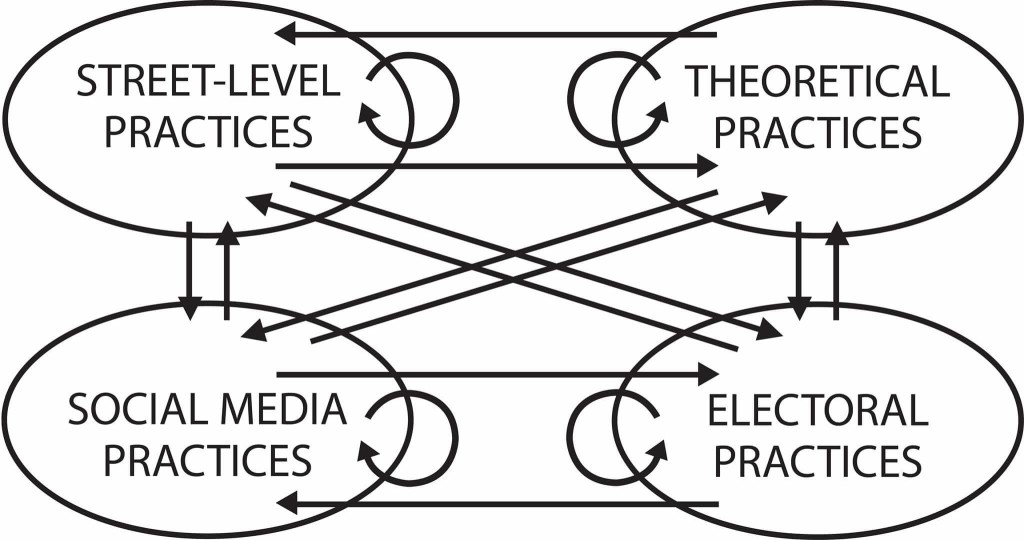
\includegraphics[width=.9\linewidth]{spheres-practices.png}
	\caption{Interacción entre prácticas electorales, teóricas, mediáticas y de calle.}
	\label{fig:interacciones}
	\todo[inline]{Valdria la pena rehacer un diagrama como este en español.}
\end{figure}

Una vez que logremos consolidar una infraestructura común y dinámicas para comunicarnos, es necesario que abramos canales de comunicación. Para lograrlo, podemos recurrir a estrategias muy antiguas, pero igualmente efectivas bajo una gran organización técnicamente capaz de hacer una democracia efectiva: Periodismo popular, repartido en lugares de resistencia a través de estructuras distribuidas por todo el país, donde los contenidos puedan enlazar realidades locales con la nacional. En realidad, la presencia de una organización política en el territorio no significa que haya buenas razones para ocuparlo, la razón por la que nos presentamos en la calle es quizá una de las cuestiones más importantes a resolver. Por ejemplo, adoptar una agenda municipalista sería un excelente horizonte para un movimiento que busca ocupar las instituciones del poder. Las propuestas de Murray Bookchin, ecologista estadounidense, pueden convivir con otros esfuerzos de organización comunitaria como los desarrollados por Saul Alisnky y Marshall Ganz. Quizá la razón más vital para salir a la calle sea la más poderosa. El carnaval, la festividad profana de lo público, la danza libre y el encuentro de los cuerpos, sería un gran pretexto. ¡Salgamos a la calle a divertirnos y hablar de lo político! También puede servir para redefinir nuestra concepción de un mercado libre y abierto.

Se pueden conciliar movimiento y elecciones a través de participación escalonada que se gestione a través de una plataforma web, así como plantear acciones importantes pero no urgentes para la organización y para desarrollar el movimiento. Esto para hacer una mancuerna operativa con las personas que consideran que conquistar espacios de poder es la tarea urgente, pero que estarían de acuerdo con abrir la organización para que están acciones importantes empiecen a ocurrir porque somos una wiki inteligente, que entiende el aspecto multidimensional de sus operaciones. Imaginamos una apertura escalonada de información, según lo que la gente quiera compartir y lo que la wiki haya ganado por su mérito de honorabilidad. \emph{Hay que entender que hoy es posible programar la gestión de responsabilidades orgánicamente.} Las alianzas deben permitirnos articular una red electoral, un plan de gobierno y un nuevo proyecto constitucional, desde una perspectiva abierta, transparente y \emph{FLOSS}. Consideremos que hay una asimetría en acceso a redes que hacen que gente menos experta o que ha pasado menos tiempo en la red tenga mayores dificultades para integrarse. Por esta razón no sabemos dar cauce a muchas ideas que son potencialmente grandes proyectos. Más allá de la preocupación porque un grupo de poder coopte la organización, hay que pensar que es necesario que el movimiento se fragmente y diferencie a partir de recursos comunes, bajo una visión modular y escalonada de los progresos de nuestra estructura política.

\begin{figure}[htbp]
	\centering
	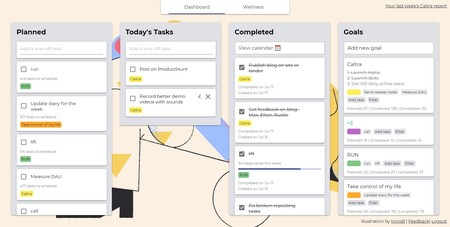
\includegraphics[width=.9\linewidth]{caltra.jpg}
	\caption{El sitio \url{www.caltra.co} te permite organizarte en listas y tableros.}
\end{figure}

El problema de la documentación de un movimiento político que busque la libertad real de todas las personas es una preocupación muy presente desde Podemos pero realmente constante a lo largo de la historia. El problema más importante hoy en día para los movimientos autogestionados se conoce como la \emph{tiranía de la no estructura.} Un problema difícil de enfrentar es que, en relación con el estado actual de las cosas, solo podemos ver lo que nos queda y muy pocas veces lo que nos ha sido arrebatado o todo lo posible, un horizonte imaginario de formas de organización, de diálogo, distintas. La cuestión de la inteligencia colectiva no puede quedarse como un instrumento más para agilizar la productividad. Mucha gente en Wikipolítica no se da cuenta lo útiles que resultan al Imperio con el burdo aceleracionismo de blancos por el que sienten tanta simpatía. Para hacer frente a estas cuestiones, necesitamos mecanismos para profesionalizar el activismo y la militancia, mecanismos de sistematización de experiencias. Partir de esto para diseñar un programa de crecimiento dirigido comprensivo y estratégico, una suerte de comunidad de inteligencia. Tenemos oportunidad de usar y desarrollar plataformas tecnológicas para gestionar procesos que ahora son inoperables bajo la tecnología que tenemos ahora. Para lanzar una campaña de crecimiento dirigida al territorio necesitamos despliegues de profesionales en Trabajo social en Comunicación. Es decir, necesitamos pensar estratégicamente. El problema es que entre muchas personas es moralmente incorrecto repetir

En Wikipolítica muchas veces nos preguntamos sobre las características de un posible espacio wiki oficial. Con el tiempo, estamos más convencidas que se trata de plantear qué significa un espacio wiki, preguntarnos cómo inspiramos a otras personas a crear espacios bajo una filosofía común. La ideología es la máscara a través de la cual vemos las cosas.

El diseño es parte de una propuesta de inteligencia que, a través de procesos de iteración y prueba, logra crear relaciones de experiencia entre las cosas y las personas. Creemos en el valor del Diseño como disciplina fundamental para la transmisión de un medio popular. Nuestro \emph{código} tiene que pensar en las instituciones a través del Diseño social. El resultado serán mecanismos que incentiven la participación más allá de la lógica utilitarista, fundamento de la magia negra. La única restricción serían las manifestaciones de totalitarismo, como la intolerancia, el autoritarismo o la intransigencia. Los discursos que atenten contra la determinación libre y voluntariosa de la persona deben ser contenidos y este es un límite al que no estamos dispuestas a renunciar.\footnote{El mejor remedio para los fascistas de sonrisa cínica y espíritu perverso es molerlos a palos. Pero nos conformamos con que sean expulsados.}

Por ejemplo, aprender a pensar en instancias para crear protocolos comunes de distintas luchas como las tecnologías de performance o la táctica del brigadeo. Operaciones orientadas a proyectos, donde las estructuras nazcan y mueran, sean ocupadas, como los hackerspaces. Metodologías de organización para y desarrollo para personas como SCRUM, design thinking, UX, grupos de agilismo, Workcafé. Otra tarea es consolidar un equipo de relatores que puedan sistematizar con rigurosidad los resultados de todas las discusiones, pues parece que la relatoría presupone más habilidades para la síntesis y la estructuración discursiva de lo que podría parecer.

La cuestión de una plataforma política puede funcionar muy bien como un proyecto modular de fuentes libres y abiertas basado en tecnologías que ya existen, como Decidim y las metodologías de gobernanza en círculos llamada Sociocracia. Con esta visión es muy factible desarrollar una estructura informática con directorios, sesiones de planificación y estrategias de mercado, asesoría para participar en convocatorias y solidaridad para que quienes quieran, se apoyen. Solo habría que considerar que el crecimiento esté dirigido estratégicamente hacia redes y personas clave en agendas específicas, además del mero crecimiento territorial. Necesitamos comprometernos con sentar un precedente operativo basado en nuestro potencial tecnológico. Si lo hacemos bien, la necesidad de apertura de otras asambleas políticas en el país se esparcirá como un meme (virus cultural), que permita que todas tengamos los saberes necesarios para organizarnos en torno a lo común.

En términos estratégicos, es mejor dar un golpe nacional de la nada, con precisión y organización, con artistas, académicos, opinión pública y otros sectores, que el desgaste que implica concentrarse en un solo proyecto de corto plazo, como una campaña política o una petición legislativa sin ninguna repercusión estructural. Mejor esperar unos años hasta que tengamos una organización poderosa. Abrir la organización con un movimiento nacional que siente las bases para un proyecto político fuerte y de larga duración.

Representación de convicciones políticas, agendas desde subjetividades reconocidas y desde los territorios. Burocracia media en sindicatos o partidos. Diferencia y relación entre sindicatos y partidos. Redes interuniversitarias. Necesitamos regulación de proyectos económicos a través de sus limitaciones. Es decir, si la industria editorial genera capital que se acumule en pocas manos (lo que significa menores ingresos tanto para escritorxs como para lectores), ser el espacio y respaldo de la innovación de nuevos modos de financiamiento, quizá haciendo hackatones o dando prioridad al tema en las agendas de un período y una región en particular. Hackatones sociales o alguna iniciativa donde podamos ser facilitadoras de distintos fondos públicos locales. En el terreno económico podemos jugar el papel de gestoras para cooperativas de consumo que compartan una identidad y principios wiki que permitan que muchas familias puedan empezar a adquirir sus bienes en redes sororas.

\section{¿Cómo entender los problemas de nuestro país?}
\label{sec:problemaspais}

El Estado en México es un orden social de acceso limitado, hay que
pensar en systems thinking para crear un frame que comprenda necesidades
para ajustar la plataforma política al contexto de institucionalidad y
reglas del juego propias de cada arreglo. Habría que partir de una
visión combinada de psicoanálisis, diseño y economía de la conducta. Hay
que hacer una lista de problemas principales a resolver, por ejemplo:

\subsection{Problemas de diseño de sistemas:}
\label{sec:probsis}

\begin{itemize}
	\item Interfaces y experiencia de usuario comunitarias y accesibles

	\item Teoría del empujón para incentivos económicos a cooperativas y apropiaciones comunitarias del espacio público
\end{itemize}

\subsection{Problemas de acción colectiva}
\label{sub:probaccion}

\subsubsection{Económicos}
\label{subs:economicos}

\begin{description}
	\item[Asimetrías de información:] cómo hacemos que la gente tenga los mismos insumos para tomar las decisiones más benéficas para las comunidades en un mercado complejo de transacciones en tiempo real

	\item[Problema del agente-principal:] abolir las altas tasas cobradas por coyotes que dan sentido a la figura del Estado como recaudador central que redistribuye el ingreso

	\item[Tiranía de la no estructura:] sistemas de toma de decisiones para la participación escalonada y remunerada de diferentes agentes con un objetivo común de solidaridad económica

	\item[Comunes:] formalización en protocolos y procesos de una cultura de los bienes y servicios comunes que se gestionan, se actualizan y se mantienen a través de contribuciones pre-establecidas en contratos inteligentes
\end{description}

\subsubsection{Psíquicos}
\label{subs:psiquicos}

\begin{description}
	\item[\emph{Schadenfreude}:] cómo crear grupos de personas con adicciones, resentimientos o comportamientos tóxicos que sienten placer por el sufrimiento del prójimo, y comenzar procesos de sanación colectiva descentralizados, como Alcohólicos Anónimos.

	\item[Narcisismo de las pequeñas diferencias:] Construcción de una cultura política que procure las alianzas y permita canalizar los disensos. Un ejemplo muy claro para la construcción de organizaciones que hagan frente a este tipo de cuestiones es la Sociocracia.
\end{description}

\begin{figure}[htbp]
	\centering
	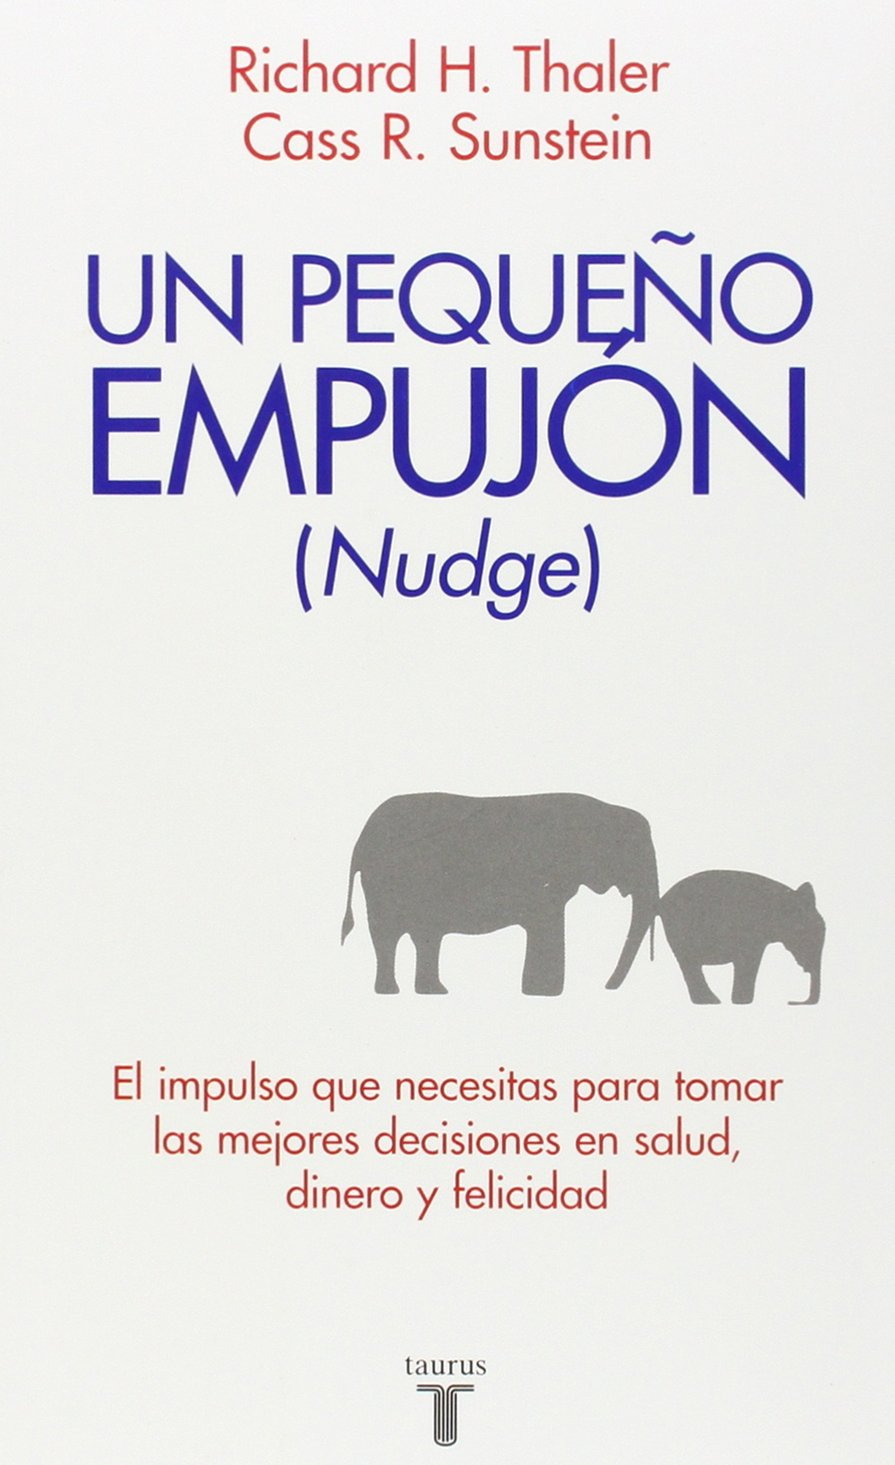
\includegraphics[width=.9\linewidth]{nudge.jpg}
	\caption[\emph{Nudge}]{El libro \emph{Nudge} es una gran referencia para entender el poder del diseño y la economía del comportamiento en la solución de problemas públicos.}
	\label{fig:nudge}
\end{figure}

\section{Consideraciones sobre la organización}
\label{sec:considerorga}

Las herramientas ya existen, es poco trabajo en interconectarlo (compatibilidad de tecnología), hay que enfocarnos en la adopción a través de talleres y eventos de accesibilidad, de editorializar una base de datos opinionated suite de trabajo militante), de garantizar protocolos de seguridad: decentralizacion, permisos (gestion de identidad) (Pursuance, sneakernet y otras tecnologías). Tenemos que desarrollarlo poco a poco a través de una arquitectura modular y distribuida, que permita ensamblar diferentes tecnologías según las necesidades de la persona usuaria.

El problema principal para un movimiento horizontal es el problema de la \emph{no-estructura}.\revquotes{} Dentro de las estrategias, podemos proponer visiones para que los emprendedores entiendan como disruptivo lo que es estructural. Se trata de reapropiarse del concepto de "gobernanza"dinámica y participativa, pensar que sea una gobernanza basada en \hlfix{outputs}{En cursivas.} o resultados sin que se vuelva una cosa individualista de \hlfix{tracking}{Ibid.} de \hlfix{performance}{Ibidem.} individual. El objetivo es crear una estructura de los comunes (Elinor Ostrom), además de fortalecer sindicatos, acelerar cooperativas y democratizar decisiones corporativas, facilitar \hlfix{self-management}{Ibid.} y \hlfix{self-organization}{Ibidem.} en un movimiento \hlfix{antileadership}{Ibid.}.

Para lograrlo hay que retomar la paradoja de la sistematización de actividades ¿creamos y documentamos procesos o patrones? ¿Realmente vale la pena un modelo de gobernanza como sociocracia?

Recursos interesantes para este apartado:

Github: The GitHub Debacle and Why Holacracy is Bullshit
(counter-response)
\url{http://cbracy.tumblr.com/post/79876957198/the-github-debacle-and-why-holacracy-is-bullshit}